\section{Magnetostatische Analyse (MS, Magnetostatic Analysis)}
Die magnetostatische Analyse basiert auf der gleichmässigen Bewegung des elektrische Stroms. Der elektrische Strom ist über die Zeit konstant. Die magnetostatische Analyse wird für die Berechnung der Ersatzinduktivität von elektrischen Komponenten gebraucht.
\subsection{Integralgleichungen}
\begin{tabular}{|p{.30\textwidth} |p{.65\textwidth}|}
	\hline 
	\textbf{Ampèresches Gesetz} \newline
	{\centering\tabbild[width=4cm]{images/ampgesetz.png}\par} & Das Ampèresche Gesetz definiert die Verteilung des magnetischen Feldes durch eine geschlossene Kurve und dem gesamten Strom durch die entsprechende Fläche
	\[ \oint\limits_{(C)}\vec{H}\cdot\vec{dl} = \iint\limits_{(A)}\vec{J}\cdot\vec{dA}\] \newline
	 \[ \oint\limits_{(C)}\vec{B}\cdot\vec{dl} = \mu_{0}\iint\limits_{(A)}\vec{J}\cdot\vec{dA}  \quad \quad\vec{B}=\mu_{0}\mu_{r}\cdot \vec{H}\]\\
	\hline
	{\centering\textbf{Durchflutungsgesetz}\par}
	& \[ \oint\limits_{(C)}\vec{H}\cdot\vec{dl} = \sum\limits_{k = 1}^{n} I_k = \theta \] 
	 \[ \oint\limits_{(C)}\vec{B}\cdot\vec{dl} = \mu_{0}\sum\limits_{k = 1}^{n} I_k = \theta \]\\
	\hline
	\textbf{Coulombsches Gesetz} \newline
	{\centering\tabbild[width=4cm]{images/quellenfreiheit.png}\par} & Der magnetische Fluss durch eine geschlossene Fläche ist immer Null. Somit sind die magnetische Feldlinien immer geschlossen. Es gibt keine magnetische Monopole. Das magnetische Feld ist quellenfrei \newline
	\[ \oiint\limits_{(A)}\vec{B}\cdot\vec{dA} = 0\]\\
	\hline
\end{tabular}
\clearpage
\pagebreak
\subsection{Differenzialgleichungen der magnetostatischen Analyse}
\begin{tabular}{|p{.45\textwidth} |p{.45\textwidth}|}
	\hline
	\textbf{Differenzialgleichung der Durchflutung}\newline
	\[\rotation \vec{H}=\nabla \times \vec{H}=\vec{J}\]
	\[\rotation \vec{B}=\nabla \times \vec{B}=\mu_{0}\vec{J}\]&
	\textbf{Vektorpotential}\newline
	\[\nabla \times \vec{A}=\vec{B} \quad\quad \nabla\cdot \vec{A} =0\]	
	\[\Delta\vec{A}=-\mu_{0}\vec{J}\]
	\[\Delta\vec{A}=0\]\\
	\hline
\end{tabular}
\subsection{Randbedingungen}
\begin{itemize}
	\item Magnetische Isolierung $\vec{n} \times \vec{A} =0$
	\item Der Rand zwischen zwei Materialien $\vec{n} \times \vec{A_{1}}=\vec{n} \times \vec{A_{2}}$
	\item Der Rand zwischen zwei Materialien $B_{1}=B_{2} \rightarrow \dfrac{dA_{1}}{d n}=\dfrac{dA_{2}}{d n} $
\end{itemize}
\subsection{Randwertproblem}
\begin{minipage}{8cm}
	\begin{itemize}
		\item $\Delta\vec{A}=-\mu_{0}\vec{J}$
		\item $\vec{n} \times \vec{A} =0$
	\end{itemize}	
\end{minipage}
\begin{minipage}{8cm}
	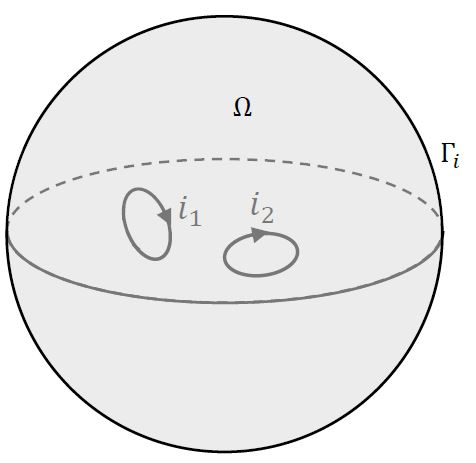
\includegraphics[width=4cm]{images/Randwertproblem.jpg}
\end{minipage}
\subsection{Vorgehen}
	\begin{enumerate}
		\item Partielle Differentialgleichung 2. Ordnung des Vektorpotentials aufstellen (Poisson oder Laplace)
		\item Koordinatentransformation wenn nötig
		\item Vereinfachung der partiellen DGL in eine gewöhnliche DGL 
		\subitem Von welcher Variable hängt das Vektorpotential ab
		\item Aufstellen der Randbedingungen
		\subitem Randwerte für Vektorpotential und B-Feld
		\item Gewöhnliche DGL 2x integrieren und nach Vektorpotential auflösen
		\item Randwerte einsetzen und unbekannte Konstanten bestimmen
	\end{enumerate}
\clearpage
\pagebreak